\chapter{Background}
\section{Compiler Correctness}
``Can you trust your compiler?''

This quote begins the paper on the CompCert project \cite{leroy2019compcert}, one of the largest proofs of compiler correctness. These proofs aim to provide trust in our compilers by formally verifying that they preserve the meaning of programs that they translate. CompCert provides such a proof for a purpose-built compiler that translates a large subset of C to machine code. For large languages like C, which have correspondingly large compilers, these proofs are notoriously difficult --- CompCert totals around 100,000 lines of code in the Coq proof assistant, and took over 6 years to complete \cite{leroy_formal_2009}.

In this section, we will review some background on compiler correctness proofs. To do so, we have to look not only at the history of such proofs themselves, but also the evolution of tooling that embeds mathematical logic systems and allow for management of large-scale proofs. Without such systems, modern, large-scale projects such as CompCert would not be possible, so the advancement of these tools is key to understanding the progression of compiler correctness proofs. 

\subsection{History}
The first known formal proof of compiler correctness comes from John McCarthy and James Painter \cite{mccarthy_correctness_1967}. In their 1967 paper, they prove that a compiler that translates simple arithmetic expressions to machine code is correct. Despite the simplicity of the example source language, the paper is very important in that it sets up a methodology for computational proofs of compiler correctness. For example, their method of proof by structural induction of expressions is still an oft-used strategy for reasoning about properties of a languages programs.

McCarthy and Painter's proof was intentionally simple, so much so that it was able to be manually formulated and checked. However, when dealing with larger languages, case analysis of language expressions quickly generates too large of a proof to keep track of by hand. Because of this complexity, modern proofs of compiler correctness universally utilize programs called proof assistants that embed mathematical logic systems and can computationally verify the consistency of theorems defined within them. These assistants are necessary to aid with management of proofs at such a large scale. As such, their creation and development has been strongly connected to the progress of compiler correctness proofs.

\subsubsection{Proof Checkers, Intuitionistic Logic, and Mechanized Proofs}\label{sxn:mech_background}
The first large-scale attempt to \textit{mechanize} mathematics, or formally define mathematics in a way tractable by a computer, was Nicolaas Govert de Bruijn's Automath language \cite{nederpelt_survey_1994}. Automath was an early example of a correspondence between logic and programs --- in the Automath language, theorems are defined as types, and proofs consist of showing that these types are inhabited by some value. This means that the definitions and proofs of theorems within Automath's logical framework are represented as a computer program. This relationship between programs and logic is also at the core of the Curry-Howard correspondence between deductive logic and the simply-typed Lambda Calculus.

Research into these sorts of program-logic relations continued into the 70s and 80s, with the development of the \textit{Intuitionistic Theory of Types} \cite{martin-lof_intuitionistic_1998} by Per Martin-Löf and the polymorphic Lambda calculus \cite{girard_interpretation_1972} by Girard. These theories also rely on the Curry-Howard correspondence to tie their dependently typed programs to statements in \textit{intuitionistic logic}. 

Intuitionistic logic is a kind of logical system that requires \textit{evidence} or \textit{witnesses} of a statement to prove its validity. That is, to prove that a statement $A \xrightarrow{} B$ is true in an intuitionistic logic, one must use the axioms of the logic to \textit{construct} evidence that B is true from the existing evidence that A is true. One important property of these intuitionistic logics that follows their constructive foundation is that the law of the excluded middle is not true in these systems --- that is, we cannot perform indirect proofs, for example by contradiction. In other words, proving that $\lnot A$ is not true does not suffice as proof of A. In this way, intuitionistic logic requires more direct proof of statements. In systems such as Automath, where a correspondence between logical statements and programs is established, a constructive proof of a statement corresponds to an algorithm that generates the program representing that statement. Because of this strong correspondence, these constructive, intuitionistic proofs lend themselves extremely well to automation, just as developers may automate complex parts of a software project.

A further example of the natural connection between intuitionistic logic and dependent type theory is Thierry Coquand's Calculus of Inductive Constructions\cite{coquand_calculus_1986, paulin-mohring_introduction_2015}. This system combines Intuitionistic Type Theory and the polymorphic Lambda Calculus into a single calculus that also provides support for writing specifications that automatically come equipped with powerful induction principles.

While the Calculus of Inductive Constructions is powerful, it is unwieldy and hard to manually construct large programs with. For this reason, the Coq proof assistant \cite{barras_coq_1997} was devised. An extension of the original Automath language, Coq embeds the Calculus of Inductive Constructions, and also provides a high level tactics language \cite{delahaye_tactic_2000} on top of the core calculus. This tactics language provides automation in the form of syntactic sugar and algorithmic search of core calculus expressions to assist in the construction of large proof terms. This tactics language greatly increase the size of proofs that Coq can handle --- indeed, Coq programmers spend the majority of their time writing, configuring, and refactoring proofs using the tactics language, so at a much higher level than using the calculus itself. 

Because of its support for automation, its history, and a large amount of libraries and community support, Coq is a natural choice for large-scale mechanized proofs. One example of this is the proof of the four color theorem. This theorem was famously unsolved until Coq's automation features made its extensive case analysis proof feasible \cite{gonthier_formal_2008}. Other projects realized in Coq include the Univalent Foundations project \cite{voevodsky_univalent_2010}, which attempts to build a foundation for mathematics based on a type theory, and the CompCert project.

Finally, while we focus on Coq because of its usage in this project, a plethora of modern proof assistants exist \cite{geuvers2009proof, barendregt2001proof}. Some examples of modern languages that are used as proof assistants include Lean \cite{de2015lean}, Agda \cite{bove2009brief}, and Idris \cite{brady2013idris}. More and more frequently, and in various fields, these tools are used to provide mechanized proofs to accompany research papers. In the next section, we will review some modern compiler correctness projects, all of which use proof assistants to validate their approach.

\subsubsection{Verified Compiler Projects}\label{sxn:new_proofs}
Table \ref{tab:cc_projs} gives an overview of some compiler verification projects.
\begin{table}[]
    \centering
    \begin{tabularx}{\textwidth}{l|X}
         CompCert \cite{leroy2019compcert} & A verified compiler from C to various assembly languages, written and proven in Coq. \\
         CakeML \cite{kumar2014cakeml} & A verified compiler for a subset of ML, verified using Isabelle/HOL \cite{nipkow2002isabelle} \\
         CertiCoq \cite{anand2017certicoq} & A verified Coq compiler, also written and proven using Coq \\
         VLISP \cite{guttman_vlisp_1995} & A verified (but not mechanized) compiler for an early version of Scheme \\
         ClightTSO \cite{sevvcik2011relaxed} & An extension of CompCert that verifies a compiler for a C-like language that supports shared-memory concurrency. \\
         Concurrent Java \cite{lochbihler2010verifying} & A verified compiler for a subset of Java that supports threading, formalized in Isabelle/HOL.
    \end{tabularx}
    \caption{Sampling of verified compiler projects}
    \label{tab:cc_projs}
\end{table}

So concludes our background on compiler verification projects and history. In the next section, we will review the Scheme language and its compiler, as background for our later proof of correctness of one of its passes.

\section{Scheme}
Scheme is a functional language based on LISP. While LISP supported functional programming (i.e. first-class functions and recursion) with a "lambda" notation \cite{mccarthy1960recursive}, Scheme was the first LISP to closely mirror the call-by-value Lambda Calculus by utilizing static scoping for its variable bindings. In addition, as Scheme evolved and added more features, its macro system, syntactic pattern matching, and homoiconity made it a language suited to modelling other programming languages. Because of this, Scheme has seen extensive use in the area of programming languages research. 

In this section, we will give some historical background on Scheme, then review the version of Scheme we chose for this project, and finally touch on the Chez Scheme compiler itself.
\subsection{Lambda Calculus, LISP, and Scheme}
The Lambda Calculus is a model which Alonzo Church and his students developed in the late 1930s \cite{church1936unsolvable} as a way to categorize a certain kind of number problem. It was later famously shown to be equivalent to Turing Machines, and together define the standard class of known computable problems \cite{sep-church-turing}. While programming languages are inherently based in computation, the Lambda Calculus was later found to be capable of simply and accurately modeling the behavior of parts of ALGOL 60 \cite{landin1965correspondence}, a programming language based on procedures.

While working on a LISP-based language for modeling actor-based concurrency \cite{sussman_first_1998}, Steele and Sussman discovered that their new language had a strong, unexpected connection with the Lambda Calculus. While LISP supported lambda notation for functions, it did not handle variable naming or scoping in the same way as Church's original model. However, as Steele and Sussman shaped their version of LISP, they found that they were able to greatly simplify the language by following the semantics of the call-by-value version of the Lambda Calculus closely. The resulting language, called Scheme, was shown to be able to effectively model a wide variety of other programming languages, while still maintaining a small size and a tidy semantics \cite{steele1978revised}. 

Because of its small size and close connection to both the well-studied Lambda Calculus and popular LISP language, Scheme saw widespread usage for research in the area of programming languages. Using Scheme's powerful pattern matching and tools for syntactic abstraction, researchers can quickly create a model of their work to accompany a more detailed paper. We use Scheme in a similar manner for our own work in this paper (see section \ref{sxn:rkt}).

Scheme has a language standard in the form of the Revised$^n$ Report on the Algorithmic Language Scheme (R\textit{n}RS). This standard defines a formal syntax and semantics for a large subset of Scheme, while leaving some areas up to the specific implementation. Our work is based on one of the more recent standards for Scheme --- R6RS \cite{sperber_revised6_2009}.

\subsection{Scheme Verification}
Along with its widespread usage in programming languages research, Scheme has itself been the target of formal verification projects. One such project, VLISP \cite{guttman_vlisp_1995}, was based on an earlier, denotational semantics for Scheme \cite{IEEE_scheme}. The initial VLISP project led to several formally verified extensions as well as explorations into representing Scheme using an operational semantics \cite{guttman_vlisp_system_1995}.

\subsection{The Chez Scheme compiler}
The Chez Scheme compiler is an optimizing compiler written in Scheme itself. It provides an implementation of Chez Scheme \cite{dybvig1983chez}, which follows the R6RS standard and adds some additional features. Notably, it is the compiler for many Scheme dialects, including the Racket language \cite{felleisen2015racket}. It notably utilizes the Nanopass framework \cite{keep2013nanopass} at its foundation. The framework provides a domain specific language embedded in Scheme, designed for quickly defining languages and translations between them. An example of a Nanopass language definition from the Chez Scheme compiler is shown in figure \ref{fig:nanopass_ex}. This example shows an intermediate language (L4) that removes set! expressions from another language that it extends (L3). We will see later that this definition corresponds to the pass that we prove correctness of (see section \ref{sxn:ca-pass}).

\begin{figure}
    \centering
    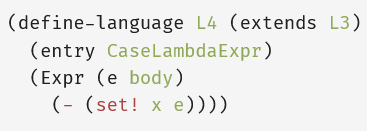
\includegraphics[scale=0.75, keepaspectratio]{figures/np_def.png}
    \caption{Example of a language definition in Nanopass}
    \label{fig:nanopass_ex}
\end{figure}

In this project, we build a framework for reasoning about Scheme and use it to prove correctness of one pass of the Chez Scheme compiler. One reason we chose to target the Chez Scheme compiler for verification was because of its usage of the Nanopass framework. Since passes are distinctly separated and small in size by design, correctness proofs of individual passes should be simpler, and also are able to be easily composed to larger proofs about correctness of a sequence of passes.
